%!TEX root = uber.tex

\section{Modeling a Strategic Driver}
\begin{frame}{Modeling a City}
\begin{columns}
\begin{column}{0.70\textwidth}
\begin{itemize}
	\item<1->\textcolor{BlueGreen}{\bf Discrete model:}
		\begin{itemize}
			\item[--]<1-> {\bf Nodes}: Set of $n$ city-zones ($\mathcal{X}$).
			\item[--]<1-> {\bf Edges}: Rides between each pair of zones.
			\item[--]<1-> {\bf Time}: advances in discrete time steps.
		\end{itemize}
	\item<2->\textcolor{BlueGreen}{\bf Empirical Transition Matrix ($F$):}
		\begin{itemize}
			\item[--]<2-> $f(i,j)$: probability of passenger in zone $i$\\ traveling to zone $j$.
		\end{itemize}
	\item<2->\textcolor{BlueGreen}{\bf Rewards Matrix ($R$):}
		\begin{itemize}
			\item[--]<2-> $r(i,j)$: net reward from zone $i$ to zone $j$.
			\item[--]<2-> $r(i,j)$ = earnings$(i,j)$ - cost$(i,j)$.
		\end{itemize}
	\item<2->\textcolor{BlueGreen}{\bf Travel Time Matrix ($T$):}
		\begin{itemize}
			\item[--]<2-> $\tau(i,j)$: travel time from zone $i$ to zone $j$.
		\end{itemize}
\end{itemize}
\end{column}
\begin{column}{0.30\textwidth}
\only<1>{
\begin{figure}[tbh]
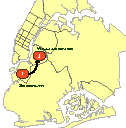
\includegraphics[scale=1.8]{figures/nyc3.pdf}
\end{figure}
}
\only<2->{
\begin{figure}[tbh]
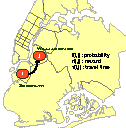
\includegraphics[scale=1.8]{figures/nyc4.pdf}
\end{figure}
}
\end{column}
\end{columns}
\vspace{0.5cm}
\uncover<3->{\alert{\textbf{In general, all these matrices are time-dependent, their entries change throughout the day.}}}
\end{frame}

\begin{frame}{Modeling a Driver}
\begin{itemize}
	\item<1->\textcolor{BlueGreen}{\bf Home Zone:}
		\begin{itemize}
			\item[--]<1-> The zone from which driver starts the day.
		\end{itemize}
		\vspace{0.25cm}
	\item<2->\textcolor{BlueGreen}{\bf Finite Horizon ($N$):}
		\begin{itemize}
			\item[--]<2->Total time steps in optimization period.
		\end{itemize}
		\vspace{0.25cm}
	\item<3->\textcolor{BlueGreen}{\bf Driving Budget ($B$):}
		\begin{itemize}
			\item[--]<3->Maximum time steps a driver is willing to drive. Obviously, $B \leq N$.
		\end{itemize}
		\vspace{0.25cm}
	\item<4->\textcolor{BlueGreen}{\bf Actions ($\mathcal{A}$):}
		\begin{itemize}
			\item[--]<4-|alert@5,6,7,8> \textbf{Get Passenger} \tikzmark{start}
			\item[--]<4-|alert@6,8> \textbf{Go Home}
			\item[--]<4-|alert@7,8> \textbf{Relocate} \tikzmark{end}
		\end{itemize}
		\uncover<5>{\naive}
		\uncover<6>{\flexible}
		\uncover<7>{\relocation}
		\uncover<8>{\flexiblerelocation}
	\item<9->\textcolor{BlueGreen}{\bf Driver Policy ($\pi$):}
		\begin{itemize}
			\item[--]<9->Time and location dependent actions takes by driver.
			\item[--]<9->Let $\Pi$ denote entire policy space of size $\big|n \times N \times B \times \mathcal{A}\big|$.
		\end{itemize}
		
\end{itemize}
\end{frame}

\begin{frame}{Problem Definition}
\begin{itemize}
	\item[] \textbf{\textsc{MaxEarnings Problem}:} Given a set of time-evolving $F, T$ and $R$ matrices, as well as the driver's budget $B$, find a policy $\pi^\ast$ such that:
	\begin{equation*}
	\pi^\ast = \argmax_{\pi \in \Pi} \mathcal{E}(\pi, F, T, R, B) 
	\end{equation*}
	where $\mathcal{E}(.)$ denotes total expected earnings.% and $\Pi$ is entire policy space $\bigg(\big||\mathcal{X}| \times N \times \mathcal{A}\big|\bigg)$.
\end{itemize}
\pause
	\only<2>{
	\begin{figure}
	\centering
	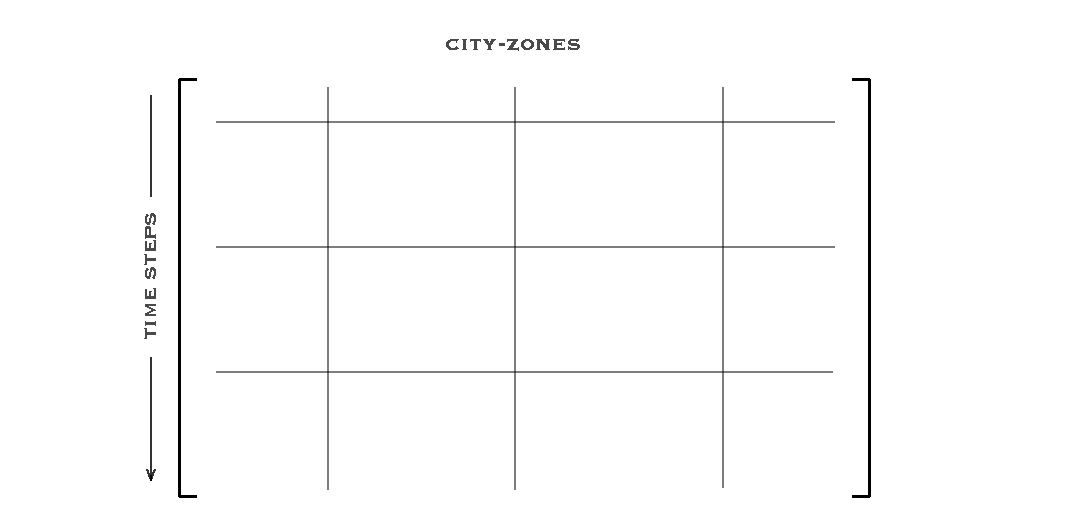
\includegraphics[scale=0.45]{figures/matrix.pdf}
	\end{figure}
	}
	\only<3>{
	\begin{figure}
	\centering
	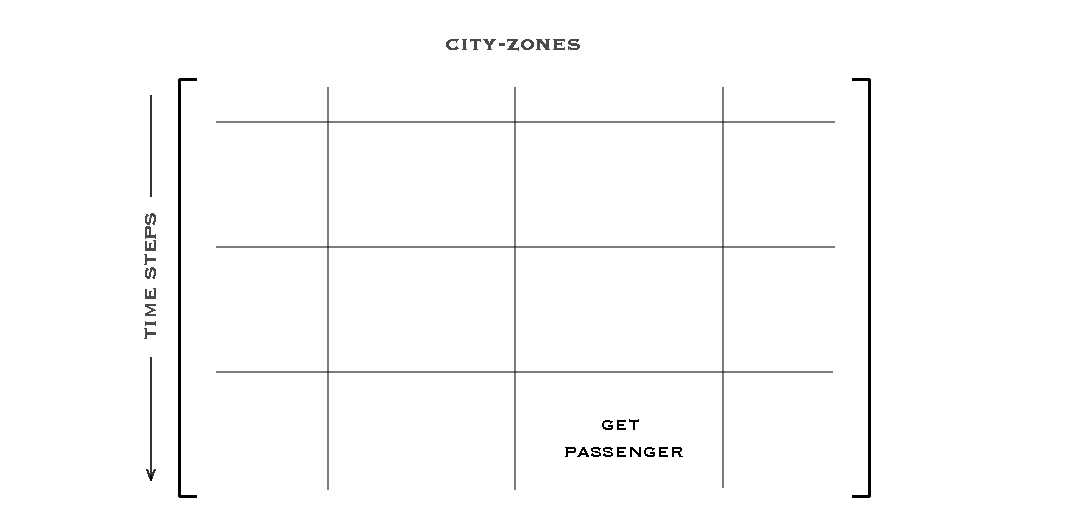
\includegraphics[scale=0.45]{figures/matrix0.pdf}
	\end{figure}
	}
	\only<4>{
	\begin{figure}
	\centering
	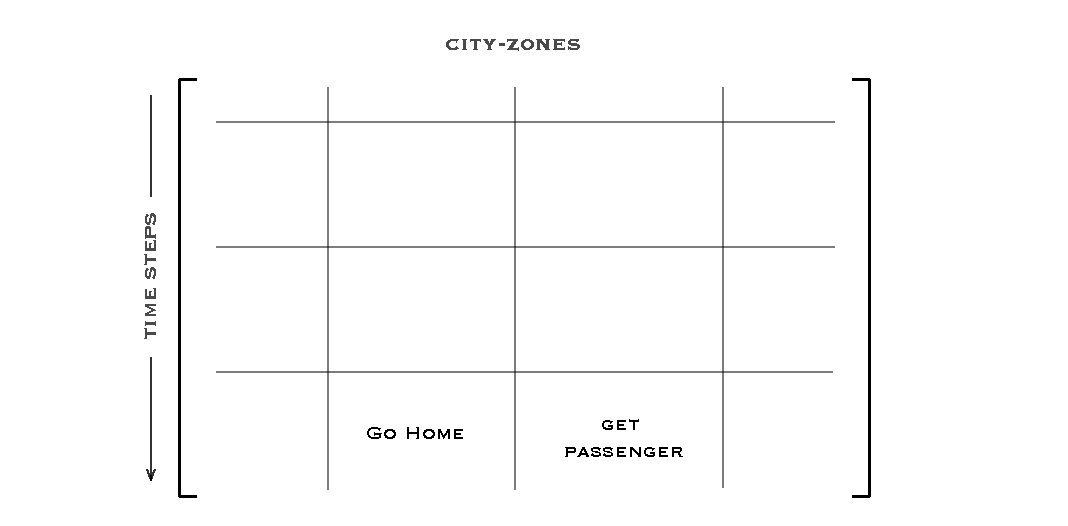
\includegraphics[scale=0.45]{figures/matrix1.pdf}
	\end{figure}
	}
	\only<5>{
	\begin{figure}
	\centering
	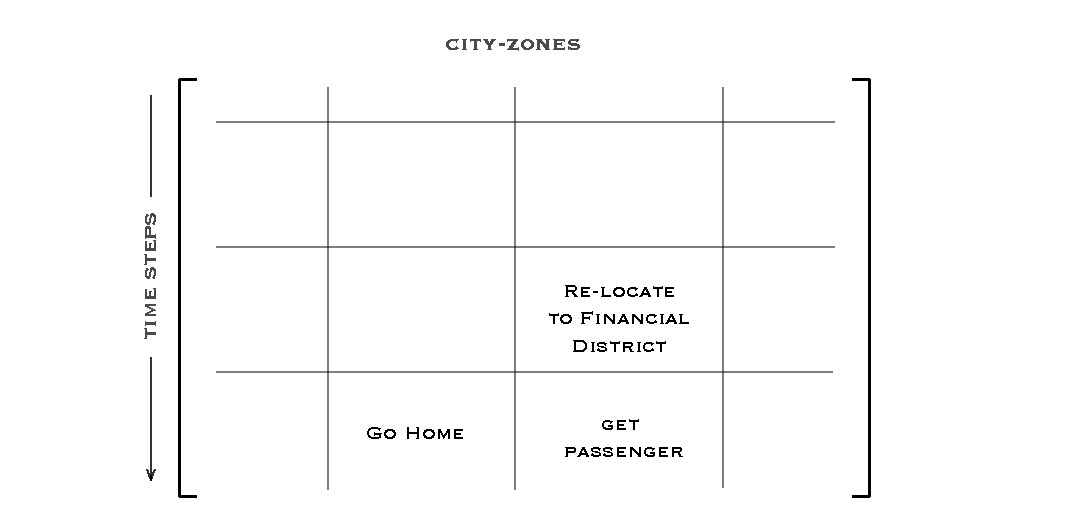
\includegraphics[scale=0.45]{figures/matrix2.pdf}
	\end{figure}
	}
	\only<6>{
	\begin{figure}
	\centering
	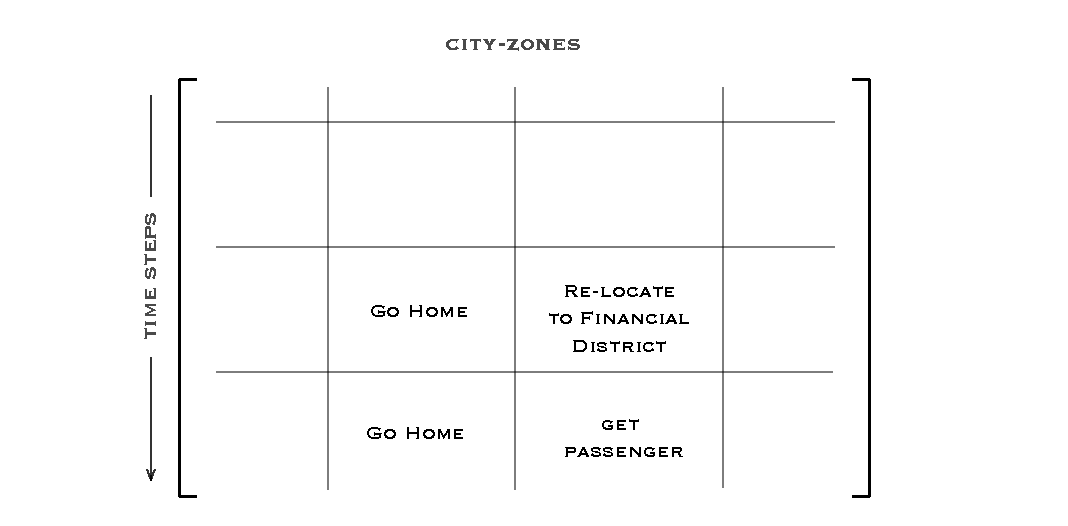
\includegraphics[scale=0.45]{figures/matrix3.pdf}
	\end{figure}
	}
	\only<7>{
	\begin{figure}
	\centering
	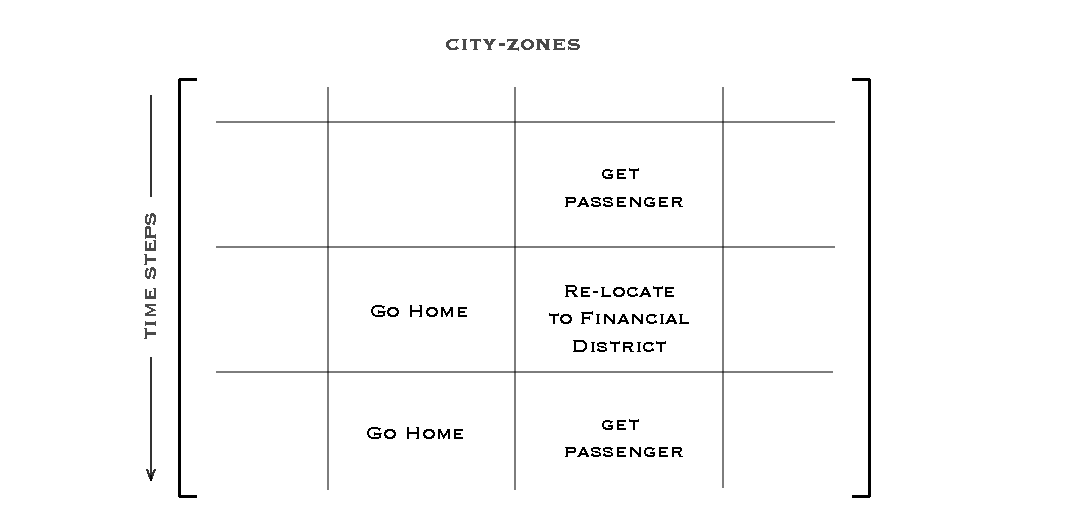
\includegraphics[scale=0.45]{figures/matrix4.pdf}
	\end{figure}
	}\only<8>{
	\begin{figure}
	\centering
	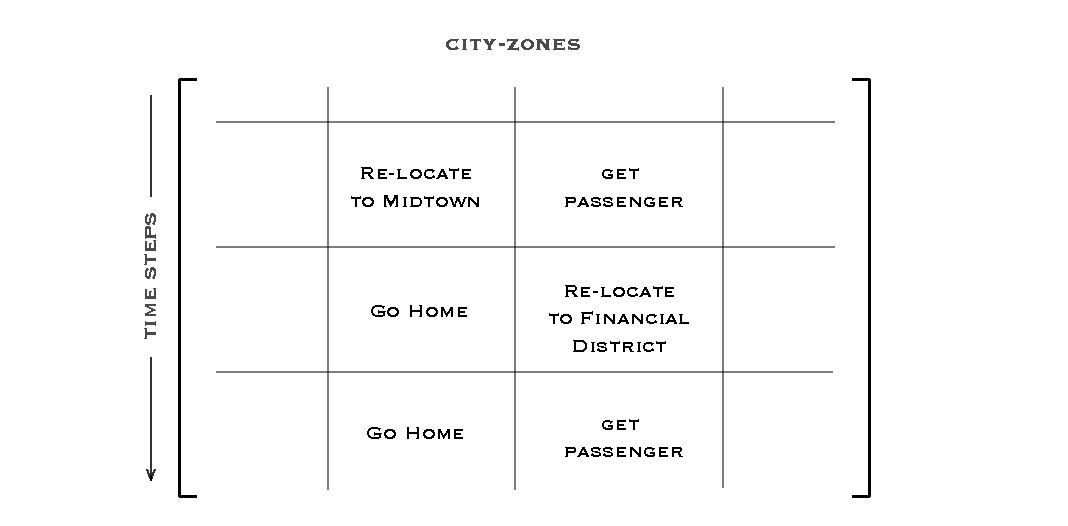
\includegraphics[scale=0.45]{figures/matrix5.pdf}
	\end{figure}
	}
	\pause
	\alert{Dynamic Program solvable in $O(n^2NB)$.}
\end{frame}